\documentclass{article}

\usepackage[T2A]{fontenc}
\usepackage[utf8]{inputenc}
\usepackage[russian]{babel}

\usepackage{amsmath}

\usepackage[unicode, colorlinks, linkcolor=blue]{hyperref}

\usepackage{graphicx}
\graphicspath{{pictures/}}
\DeclareGraphicsExtensions{.pdf,.png,.jpg}

\usepackage{pgfplots}
\usepackage{tikz}


\begin{document}
%----------------------------------Шапка---------------------------------------------
\begin{center}
	
\includegraphics[scale=0.25]{AU}\\
	{\Large\bfseries Санкт-Петербургский национальный исследовательский Академический университет имени Ж.И.~Алфёрова Российской академии наук}
\end{center}

\begin{center}
	Свиридов Фёдор, Александр Слободнюк, Владимир Попов
\end{center}
\rule{12cm}{0.4mm}
\begin{center}
	{\large\textbf{Рабочий протокол и отчёт по лабораторной работе № 5}}
\end{center}
%--------------------------------------------------------------------------------------
\paragraph{Цель работы.}
Вычислить момент инерции маятника Обербека

\paragraph{Задачи, решаемые при выполнении работы.}
\begin{itemize}
	\item Измерить массы грузов
	\item Измерить диаметр шкива
	\item Измерить высоту, с которой опускаются грузы
	\item Измерить время, за которое опускаются грузы с различной массой (маятник без грузов)
	\item Найти зависимость $\varepsilon(m)$ и с помощью экстраполяции определить $m_o$
	\item Вычислить момент инерции маятника без грузов
	\item Вычислить момент инерции маятника с грузами при различных расстояниях $r$
	\item Сделать выводы
\end{itemize}

\paragraph{Объект исследования.}
Аддитивность момента инерции $I$

\paragraph{Метод экспериментального исследования.}
Измерение момента инерции

 \paragraph{Рабочие формулы и исходные данные.}\hypertarget{formuls}{}
 \begin{equation}
 	\fbox{$I=\frac{g D^2}{8x}(m-m_0)t^2$}
 \end{equation}

\begin{equation}
	\varepsilon=\frac{4x}{Dt^2}
\end{equation}

\begin{equation}
	\Delta \varepsilon=\sqrt{\frac{16}{D^2t^4}\Delta x^2+\frac{16x^2}{D^4t^4}\Delta D^2+\frac{64x^2}{D^2t^6}\Delta t^2}
\end{equation}

\begin{equation}
	M_{\mbox{сопр.}}=\frac{m_0gD}{2}
\end{equation}

\begin{equation}
	I=\tilde{I}+4\overline{m}_1r^2
\end{equation}
где $\tilde{I}$ - момент инерции барабана; $D$ - диаметр шкива; $x$ - высота, с которой спускается груз; $ t $ -время спуска груза; $m$ - масса спускаемого груза; $m_0$~-~масса груза, которая компенсирует момент силы трения (определяется косвенно)



\begin{table}[h]
	\caption{\bf Измерительные приборы}
	\begin{tabular}[c]{|p{7.5em}|p{7.5em}|p{7.5em}| p{7.5em}|}
		\hline
		Наименование & Тип прибора & Используемый диапазон & Погрешность прибора\\\hline
		Линейка & Аналоговый & $5 - 60\quad\mbox{см}$ & 0,1 см\\
		\hline
		Штангенциркуль& Цифровой&$50-70\quad\mbox{мм}$&0,02 мм\\
		\hline
		Электронные весы& Цифровой & $1 - 150\quad\mbox{г}$ & 0,01 г \\
		\hline
	\end{tabular}
\end{table}

\begin{figure}[htb]
	\caption{\bf Схема установки}
	\centering 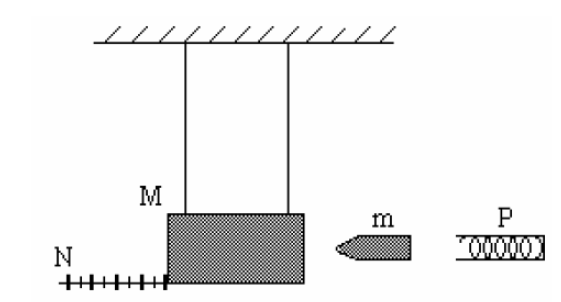
\includegraphics[scale=0.5]{схема}
\end{figure}


\paragraph{Результаты прямых измерений и их обработки.}
\begin{itemize}
	\item $ D=63,37\;\mbox{мм} $
	\item $ x=45,5\;\mbox{см} $
	\item Средняя масса грузов, которые крепятся на стержнях:\\
	$ \overline{m}_1 = 115,16\;\mbox{г}$
	\item Маятник без грузов на стержнях
	
	\begin{tabular}{c|c}
		
		$m$, г& $t$, с \\
		\hline
		46,45& 5,356 \\
		
		95,75& 3,847 \\
		
		145,05& 3,140 \\
		
		194,35& 2,785 \\
	\end{tabular}
\item Маятник с грузами $\overline{m}_1$ на стержнях, расположенные на расстояние $r$ от оси вращения:

\begin{tabular}{c|c|c}

	$r$, см&$m$, г& $t$, с \\
	\hline
	27&95,75  &6,941  \\
	22&95,75  &6,142  \\
	17&95,75  &5,063  \\
	
\end{tabular}


\end{itemize}

\paragraph{Погрешности измерений.}
\begin{itemize}
	\item $\Delta m = 0,01\;\mbox{г}$
	\item $\Delta t = 0,001\;\mbox{c}$
	\item $\Delta x = 1\;\mbox{см}$
	\item $\Delta D = 0,02\;\mbox{мм}$
	\item $\Delta r = 1\;\mbox{см}$
\end{itemize}

\paragraph{Расчет результатов косвенных измерений.}

\begin{itemize}
	\item {\bf Вычисление $\bf m_0$}
	
	
\begin{itemize}
	\item Пользуясь \hyperlink{formuls}{формулой (2)}, находим $\varepsilon$:
	
	$$\varepsilon_1=\frac{4\cdot0,455}{63,37\cdot10^{-3}\cdot(5,356)^2}\approx1\;\left( \mbox{с}^{-2} \right) $$
	$$\varepsilon_2=\frac{4\cdot0,455}{63,37\cdot10^{-3}\cdot(3,847)^2}\approx1,94\;\left( \mbox{с}^{-2} \right) $$
	$$\varepsilon_3=\frac{4\cdot0,455}{63,37\cdot10^{-3}\cdot(3,140)^2}\approx2,91\;\left( \mbox{с}^{-2} \right) $$
	$$\varepsilon_4=\frac{4\cdot0,455}{63,37\cdot10^{-3}\cdot(2,785)^2}\approx3,7\;\left( \mbox{с}^{-2} \right) $$

	\item Пользуясь \hyperlink{formuls}{формулой (3)}, находим погрешность $\Delta \varepsilon$:
	
	\begin{tabular}{c|c}
		№ & $\Delta \varepsilon,\;\mbox{c}^{-2}$ \\
		\hline
		1 &  0,02\\
		
		2 &  0,04\\
		
		3 &  0,06\\
		
		4 &  0,08\\
	\end{tabular}\\

\item В итоге:

	\begin{tabular}{ c | c | c}
		№	& $m$, г& $\varepsilon$, $\mbox{с}^{-2}$ \\
		\hline
		1 & $46,45\pm0,01 $ &  $  1,00\pm0,02  $\\
		
		2& $ 95,75\pm0,01$ & $ 1,94\pm0,04  $ \\
		
		3& $145,05 \pm0,01 $&  $ 2,91 \pm0,06 $\\
		
		4& $ 194,35\pm0,01 $& $  3,70 \pm0,08$
	\end{tabular}\\

\item С помощью метода наименьших квадратов находим $m_0$:
$$ f(k, b)=\left( \varepsilon_1-(km_1+b)\right) ^2+\left( \varepsilon_2-(km_2+b)\right) ^2+\left( \varepsilon_3-(km_3+b)\right) ^2+\left( \varepsilon_4-(km_4+b)\right) ^2$$
\begin{equation*}
	\begin{cases}
		\frac{\partial f}{\partial k}=-2m_1( \varepsilon_1-km_1-b) - 2m_2( \varepsilon_2-km_2-b) - 2m_3( \varepsilon_3-km_3-b) - 2m_4( \varepsilon_4-km_4-b) =0\\
		\frac{\partial f}{\partial b}=-2( \varepsilon_1-km_1-b) - 2( \varepsilon_2-km_2-b) - 2( \varepsilon_3-km_3-b) - 2( \varepsilon_4-km_4-b) =0
		
	\end{cases}
\end{equation*}

\begin{equation*}
	\begin{cases}
		2(m_1\varepsilon_1+m_2\varepsilon_2+m_3\varepsilon_3+m_4\varepsilon_4)-2k(m_1^2+m_2^2+m_3^2+m_4^2)-2b(m_1+m_2+m_3+m_4)=0\\
		2(\varepsilon_1 + \varepsilon_2 + \varepsilon_3 + \varepsilon_4)-2k(m_1+m_2+m_3+m_4)-8b=0
	\end{cases}
\end{equation*}

\begin{equation*}
	\begin{cases}
		(2,75\pm0.03)-(0,140274\pm0,000019)k-(0,96320\pm0,00008)b=0\\
		(19,1\pm0,4)-(0,96320\pm0,00008)k-8b=0
	\end{cases}
\end{equation*}

\begin{equation*}
	\begin{cases}
	k = 18,5297\pm2,3345\\
	b=0,1565\pm0,3246
\end{cases}
\end{equation*}

\begin{figure}[!htb]
	\centering
	\caption{Экстраполяция зависимости $\varepsilon(m)$}
\begin{tikzpicture}
	\begin{axis} [legend pos = north west, xlabel=$m{,}\;\mbox{кг}$, ylabel=$\varepsilon(m){,}\quad\mbox{с}^{-2}$]
		
		\legend{,$18.5297x + 0.1565$}
		\addplot [mark = *,only marks] coordinates {
			(0.04645,1) 
			(0.09575,1.94) 
			(0.14505,2.91) 	
			(0.19435,3.7)		
		};
	\addplot [draw=red][domain=0:0.2]{18.5297*x + 0.1565};
	\end{axis}
\end{tikzpicture}
\end{figure}

$$ m_0=-\frac{b}{k}$$

 \begin{equation*}
	\fbox{$ m_0= ({-}8\pm18)\cdot10^{-3}\;\mbox{кг}$}
\end{equation*}
По \hyperlink{formuls}{формуле (4)}:\\

$M_{\mbox{сопр.}}= ({-}2\pm6)\cdot10^{-3}\;\;\mbox{Н}\cdot\mbox{м}$
\end{itemize}
\item {\bf Момент инерции барабана $\tilde{I}$} \hyperlink{formuls}{(1)}:\\

\begin{tabular}{c|c||c||}
	
	$m$, г& $t$, с &$\tilde I{,}\;\mbox{кг}\cdot\mbox{м}^2$\\
	\hline
	46,45& 5,356& $(17\pm6)\cdot10^{-3}$\\
	
	95,75& 3,847 &$(17\pm3)\cdot10^{-3}$\\
	
	145,05& 3,140& $(16\pm2)\cdot10^{-3}$\\
	
	194,35& 2,785& $(17\pm2)\cdot10^{-3}$\\
\end{tabular}

$\tilde{I}\approx(17\pm6)\cdot10^{-3}\;\mbox{кг}\cdot\mbox{м}^2$
\end{itemize}

\paragraph{Окончательные результаты.}
\begin{itemize}
	\item Момент инерции маятника по \hyperlink{formuls}{формуле (5)}:\\
	
Таблица 2\\
	\begin{tabular}{|c|c|}
		\hline
		$r$, см&  $I{,}\;\mbox{кг}\cdot\mbox{м}^2$\\
		\hline
		27& $(5\pm0,8)\cdot10^{-2}$ \\
		
		22&  $(4\pm0,8)\cdot10^{-2}$\\
	
		17&  $(3\pm0,8)\cdot10^{-2}$\\
		\hline
	\end{tabular}\\

	\item Момент инерции маятника по \hyperlink{formuls}{формуле (1)}\\

Таблица 3\\
	\begin{tabular}{|c|c|}
		\hline
		$r$, см&  $I{,}\;\mbox{кг}\cdot\mbox{м}^2$\\
		\hline
		27& $ (5,4\pm0,8)\cdot10^{-2}$ \\
		
		22&  $ (4,2\pm0,7)\cdot10^{-2}$\\
		
		17&  $ (2,9\pm0,5)\cdot10^{-2}$\\
		\hline
	\end{tabular}
\end{itemize}

\begin{figure}[htb]
	\centering
\begin{tikzpicture}
	
		\begin{axis}
			[
			legend pos = north west,ymin=2,xmin=16,xmax=28, ymax=6.5,xlabel=$r{,}\;\mbox{см}$, ylabel=$I{,}\;\mbox{кг}\cdot\mbox{м}^2\cdot10^{-2}$,ymajorgrids
			]
			\legend{Таблица 2,Таблица 3};
			\addplot [ only marks, mark=*, error bars/.cd, y dir=both, y explicit
			]
			table [x=x, y=y, y error=y-err]
			{
				x     y  y-err
				27  5   0.8
				22  4   0.8
				17   3   0.8
			};
		
		\addplot [ color=red, only marks, mark=square*, error bars/.cd, y dir=both, y explicit]
		table [x=x, y=y, y error=y-err]
		{
			x 	     y      y-err
			27   5.4     0.8
			22   4.2     0.7
			17    2.9     0.5
		};
		\end{axis}
\end{tikzpicture}
\end{figure}

\paragraph{Выводы и анализ результатов.}
Мы измерили момент инерции маятника Обербека двумя способами, пользуясь \hyperlink{formuls}{формулами (1) и (5)}. И, к счастью, погрешности этих значений перекрываются. Это означает, что формула \hyperlink{formuls}{(5)} верна по отношению к формуле \hyperlink{formuls}{(1)}, а из этого следует, что момент инерции~-~аддитивная величина. 

В наших вычислениях встречается одна неприятность: $m_0$ имеет отрицательное значение. Так выходит из-за того, что экстраполируя $m_0$ получается большая погрешность, и вдобавок момент силы сопротивления очень мал, около $2\cdot10^{-3}\;\mbox{Н}\cdot\mbox{м}$ (соответственно $m_0$ в окрестности нуля).

Замечание по поводу нахождения погрешности: чтобы упростить арифметические вычисления для расчёта погрешности суммы $f=x+y$, мы использовали следующую формулу: $\Delta f=\Delta x + \Delta y$, вместо $\Delta f = \sqrt{(\Delta x)^2 + (\Delta y)^2 }$
\end{document}




